\documentclass{chi2009}
\usepackage{times}
\usepackage{url}
\usepackage{graphics}
\usepackage{color}
\usepackage{wrapfig}
% \usepackage{picins}
% \usepackage{floatflt}
\usepackage[pdftex]{hyperref}
\hypersetup{%
pdftitle={Mashing the Ideas Expressed on the Web},
pdfauthor={Beth Trushkowsky and Rob Ennals},
pdfkeywords={CSCW, sensemaking, web, browsers, collaboration, mind mapping},
bookmarksnumbered,
pdfstartview={FitH},
colorlinks,
citecolor=black,
filecolor=black,
linkcolor=black,
urlcolor=black,
breaklinks=true,
}

\newcommand{\todo}[1]{}
% \newcommand{\todo}[1]{\footnote{{\bf TODO:} #1}}
\newcommand{\Intel}{Intel\textsuperscript{\textregistered}}

\newcommand{\idea}[1]{{\color{blue} IDEA: #1}\\}
\newcommand{\studyresult}[1]{{\color{red} STUDY RESULT?: #1}\\}
\newcommand{\howmany}{{\color{red} (HOW MANY?)}}

\pagenumbering{arabic}  % Arabic page numbers for submission.  Remove this line to eliminate page numbers for the camera ready copy


\begin{document}
% to make various LaTeX processors do the right thing with page size
\special{papersize=8.5in,11in}
\setlength{\paperheight}{11in}
\setlength{\paperwidth}{8.5in}
\setlength{\pdfpageheight}{\paperheight}
\setlength{\pdfpagewidth}{\paperwidth}
%
\toappear{Submitted for review to CHI 2009.}

\title{Participatory Mashups: Using Users to make Data Mashable}

\numberofauthors{2}

%\author{
%	\alignauthor Authors anonymized for submission
%}

\author{
\alignauthor Rob Ennals\\
       \affaddr{Intel Research}\\
       \affaddr{2150 Shattuck Avenue}\\
       \affaddr{Penthouse Suite}\\
       \affaddr{Berkeley, CA 94704, USA}\\
       \email{robert.ennals@intel.com}
\alignauthor Beth Trushkowsky\\
       \affaddr{Computer Science Division}\\
       \affaddr{University of California at Berkeley}\\
       \email{trush@berkeley.edu}
}
\sloppy 

\maketitle

\begin{abstract}
Most mashups produced so far have concerned themselves with structured machine readable, generated from databases, or written in very standard formats. Addresses, phone numbers, products, personal profiles, information available through APIs, and information that can be scraped from well-understood web site templates.

However much of the most interesting information on the web is not in forms that a computer can easily understand. It may be in natural language text, or it may be in web site templates that our tool does not yet understand.

In this paper, we discuss the alternative approach of ``participatory mashups'' in which the users of the mashup also teach the mashup ways that it can understand new data. As examples, we present our work on Think Link, which connects factual statements on the web to related statements elsewhere, and Mash Maker, which attempts to understand the meaning of structured data on arbitrary web pages.
\end{abstract}


\section{Introduction}

If we understand what the information on a page means, then we can do useful things with it. We can connect the information to information elsewhere that might be relevant, we can compute new information from the information we have, and we can present users with new interfaces that are more powerful than that provided by any individual site.

Some kinds of information are easier to understand than others, and mashups have so far understandably focussed on the low-hanging fruit. Addresses follow an easily recognized pattern, and have led to a large number of useful mashups which plot various things on maps or work out what things are near to other things. Similarly, many mashups have made use of data that is available from APIs, or that can be easily scraped from web pages that have been generated from databases.

However much of the most interesting information on the web does not have a form that can be easily mashed up. 

Most mashups produced so far have concerned themselves with structured machine readable, generated from databases, or written in very standard formats. Addresses, phone numbers, products, personal profiles, and information laid out from standard templates. 

But a lot of the most interesting information on the web isn't like this. Much of the web consists of information written as unstructured natural language text. Arguments, ideas, opinions, factual claims, jokes. Information that cannot be easily be accessed using an API or a screen scraper.

We believe that people have the potential to benefit a lot by applying mashups to such data, understanding, connecting, and visualizing it in new ways. What other web sites oppose this opinion? What ideas would I need to understand in order to understand this idea? Do by friends agree with this? Is there a more respectable source that also voices this idea?

In this paper we discuss our work with Think Link, a tool that allows user to identify factual claims made in documents, and uses this to connect web pages to other web pages that make related claims.



People have created 


 The information on one web page can be connected to information on other web pages, structural proper


\begin{figure}[tb]
	\begin{center}
	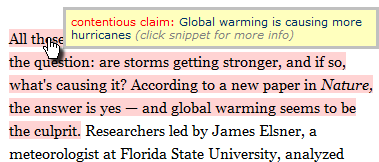
\includegraphics[width=6cm]{../screenshots/highlight_crop.png}
	\caption{Hovering over a highlighted snippet shows a summary}
	\label{highlight}
	\end{center}
\end{figure}

\begin{figure}[tb]
	\begin{center}
	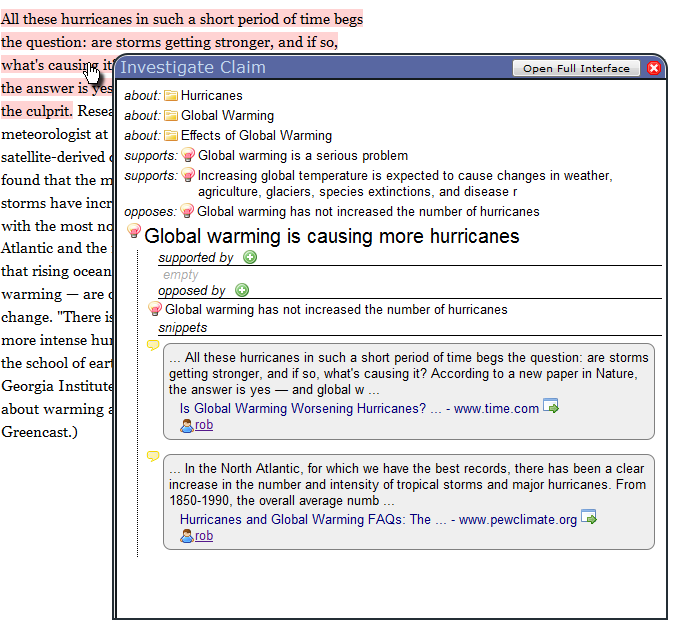
\includegraphics[width=6cm]{../screenshots/claim_popup_crop2.png}
	\caption{Click on a claim to investigate evidence for and against it}
	\label{claimview}
	\end{center}
\end{figure}

\begin{figure}[tb]
	\begin{center}
	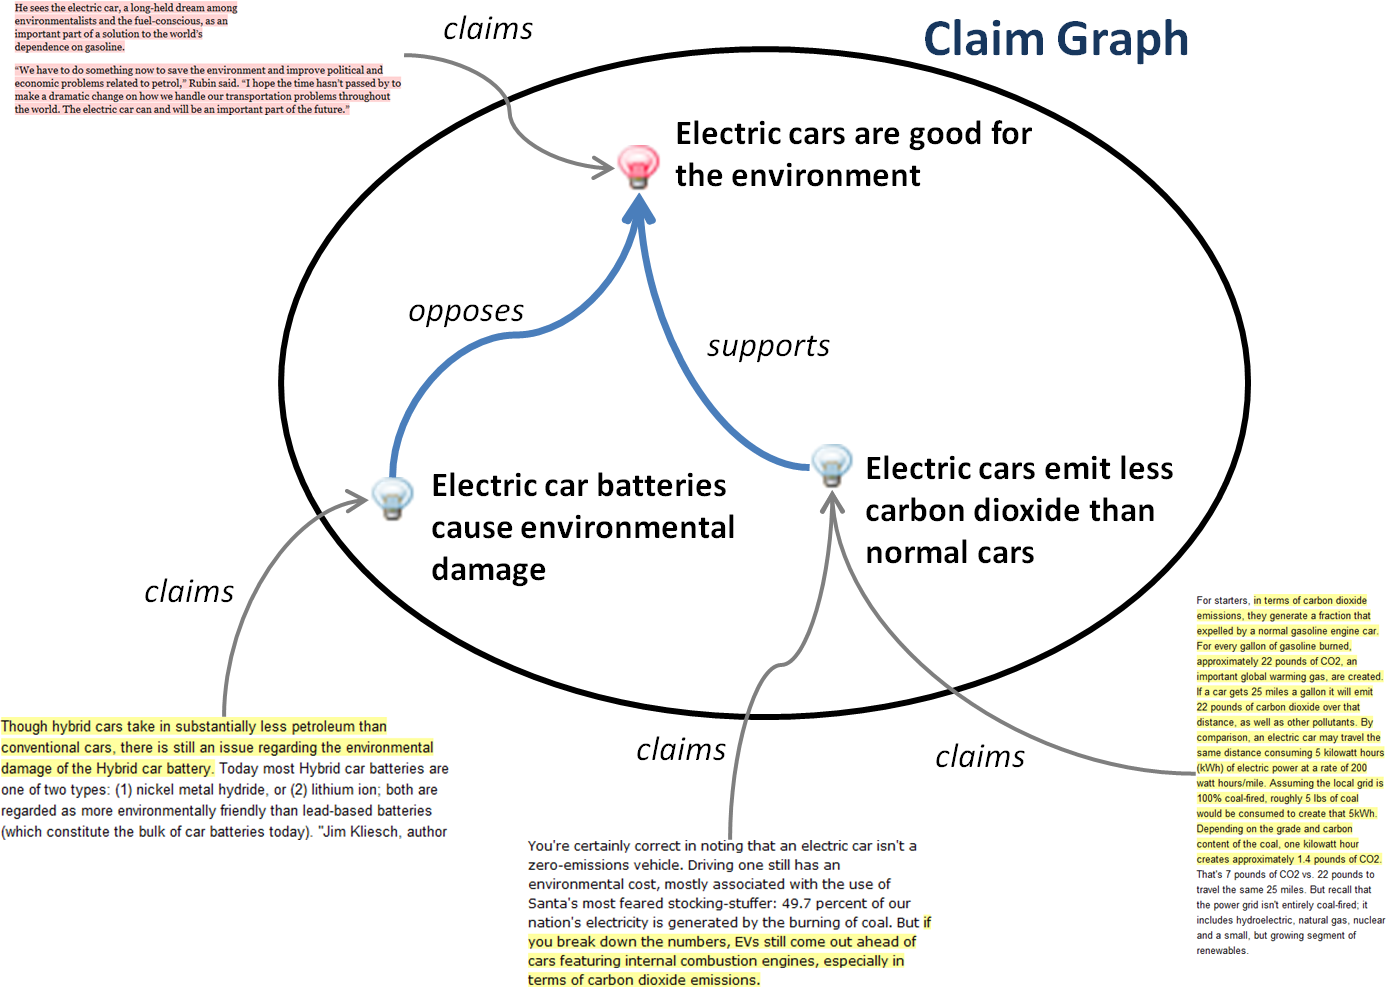
\includegraphics[width=7.7cm]{../screenshots/summary_graph.png}
	\caption{Think link connects claims to each other and to web snippets}
	\label{summarygraph}
	\end{center}
\end{figure}

\begin{figure}[tb]
	\begin{center}
	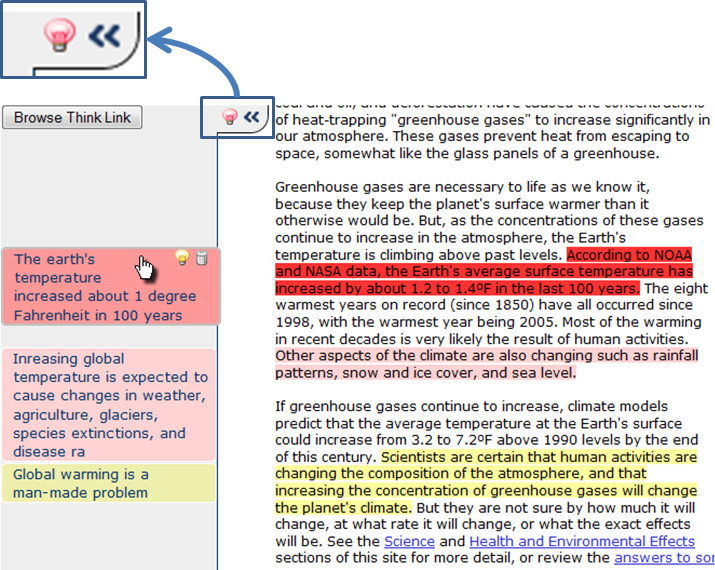
\includegraphics[width=6cm]{../screenshots/sidebar_diagram.png}
	\caption{The margin summarizes the key claims on the page}
	\label{margin}
	\end{center}
\end{figure}


\begin{figure}[tb]
	\begin{center}
	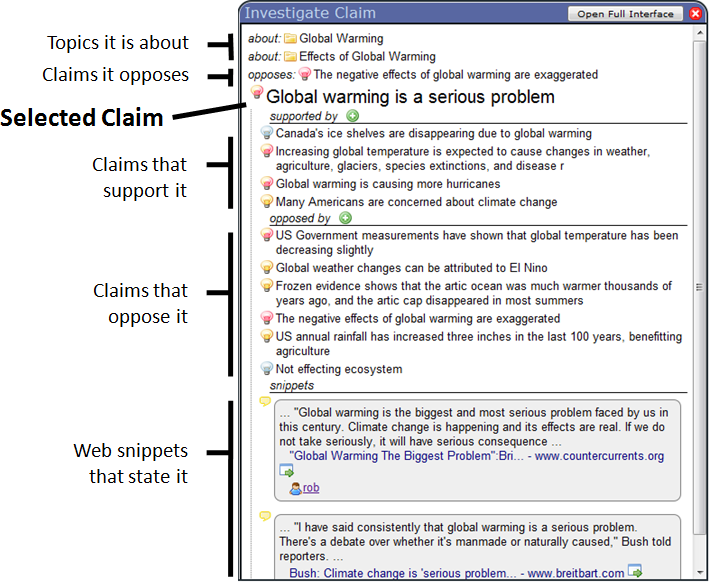
\includegraphics[width=8cm]{../screenshots/claimbrowse_diagram.png}
	\caption{The claim browser visualizes the claim graph}
	\label{claimbrowse_diagram}
	\end{center}
\end{figure}

\begin{figure*}[tb]
	\begin{center}
	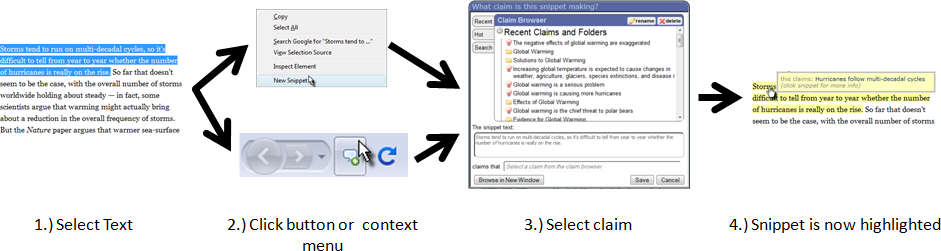
\includegraphics[width=16cm]{../screenshots/newsnip_all.png}
	\caption{Process for creating a new snippet}
	\label{createprocess}
	\end{center}
\end{figure*}

\section{Acknowledgments}

We would like to think Allison Woodruff, Tye Rattenbury, and all our user study participants for all their help during the design of Think Link. Think Link uses icons from the free FamFamFam Silk~\cite{silkicons} collection.

\bibliographystyle{abbrv}
\bibliography{biblio}

\end{document}

